%% Hello emacs, this is -*- latex -*-
\typeout{ ====================================================================}
\typeout{ This is file atlas.tex, created at 13-Feb-2004 }
\typeout{ Maintained by Andre DOS ANJOS <Andre.dos.Anjos@cern.ch> }
\typeout{ ====================================================================}

\chapter{O Experimento ATLAS no CERN}
\label{chap:atlas}

% advocate: CERN um centro de grandes pesquisas e pesquisadores.
% Alguns Premios Nobel foram executados no CERN, o que o classifica como
% um grande centro de pesquisa.

O experimento \idx{ATLAS} é um dos 4 experimentos que estão sendo construídos
ao redor do super-acelerador e colisionador de partículas \idx{LHC} (do inglês
\idxeng{Large Hadron Collider}), no Laboratório Europeu para a Física de
Partículas - \idx{CERN} em Genebra, Suíça \cite{atlas-tp}. O \idx{CERN} é um
dos maiores, senão o maior laboratório para a Física de Altas Energias na
atualidade, conduzindo vários experimentos em regime de colaboração
internacional. A próxima seção introduz um pouco de sua história, que culmina
na aprovação para criação do LHC e dos 4 grandes experimentos montados a
partir de sua infraestrutura.

\section{O Laboratório CERN}

O CERN surgiu em 1952 quando, depois de várias reuniões, 11 Estados europeus
aceitaram organizar um Conselho Europeu para a Pesquisa Nuclear (do francês
\idxfr{Conseil Européen pour la Recherche Nucléaire}) Provisório, com sede
prevista em um local próximo à Genebra, na Suíça. Dois anos após a ratificação
de uma conversão por seus \idx{Estados-Membro}, no dia 29 de Maio de 1954, o
centro era inaugurado. Embora o termo ``Provisório'' tenha sido banido do nome
do laboratório, a sigla CERN continuou a ser empregada.
 
O primeiro acelerador do CERN\index{CERN!primeiro acelerador}, um
\idxeng{Synchro-Cyclotron} de prótons a 600 MeV, começou a operar em
1957. Este acelerador foi responsável pela obtenção do primeiro resultado
experimental do laboratório: a observação do decaimento de um píon em um
elétron e um neutrino. Em 1959, a primeira ``grande'' máquina do CERN já
estava em operação. Era um \idxeng{Proton Synchrotron} (PS) de 28 GeV - o
acelerador de maior energia na época.

Algumas das tecnologias para colisão e deteção de partículas existentes nos
dias de hoje foram inventadas neste laboratório. Dentre as principais, podemos
destacar:

\begin{itemize}
\item \idx{Técnica de Resfriamento Estocástico} (do inglês
\idxeng{Stochastic Cooling Technique}), proposta por Simon van der Meer em
1968;

\item as \idx{Câmaras Proporcionais Multifio} (do inglês
\idxeng{Multiwire Proportional Chambers}) e as \idx{Câmaras de Arrasto} (do
inglês \idxeng{Drift Chambers}). A criação desta tecnologia daria o Prêmio
Nobel a Georges Charpack em 1992;
\end{itemize}

Outras tecnologias associadas também tiveram destaque. Por exemplo, em 1990,
Tim Berners-Lee, trabalhando em conjunto com Robert Cailliau, propôs um
sistema de informação distribuída, baseado em ``hipertextos'', uma forma de
descrever ligações a documentos guardados em computadores. Escondendo o
endereço de rede através de ítens grafados na tela, a informação pode ser
ligada através de vários computadores. O nome \idx{Word-Wide Web} foi
escolhido na ocasião.

A injeção de fundos para a pesquisa nuclear alavancou a criação de uma grande
infra-estrutura de anéis de acelaração e estocagem de partículas na década de
60, dos quais o mais importante aparato foi o \idxeng{Super Proton
Synchrotron} (\idx{SPS}), que começou a operar em 1976 com energia inicial de
300 GeV. O SPS têm 7 km de extensão e atravessa a fronteira franco-suíça nos
arredores de Genebra, tendo sido o maior instrumento científico da época.  A
histórica descoberta dos bósons W e Z em janeiro e maio de 1983
respectivamente ficou por conta dos trabalhos no SPS, confirmando a
\idx{teoria eletrofraca}, que unificava as forças fraca\index{força fraca} e
eletromagnéticas\index{força eletromagética}. Carlo Rubia e Simon van der Meer
receberam o prêmio Nobel por este trabalho em 1984. Este trabalho motivou a
construção do \idx{Grande Colisionador Elétron-Pósitron} (do inglês
\idxeng{Large Electron-Positron Collider}, \idx{LEP}), com energia incial
prevista para 50 GeV. O LEP estudaria em detalhes as partículas Z em quatro
experimentos simultâneos.

Os anos de 1989 a 1994 foram marcados pelo sucesso dos experimentos no LEP. O
resultado mais impressionante se deu com a precisa medição dos parâmetros de
ressonância da partícula Z: os 4 experimentos do LEP reconstruíram mais de 10
milhões de decaímentos desta partícula no período. Com base nestes resultados,
o Conselho dos Estados-Membro aprovou a construção do \idx{Grande Colisionador
de Hádrons} (do inglês \idxeng{Large Hadron Collider}, LHC). A
Figura~\ref{fig:accel} mostra o atual conjunto de aceleradores do CERN e suas
interconexões.

\begin{figure}
\begin{center}
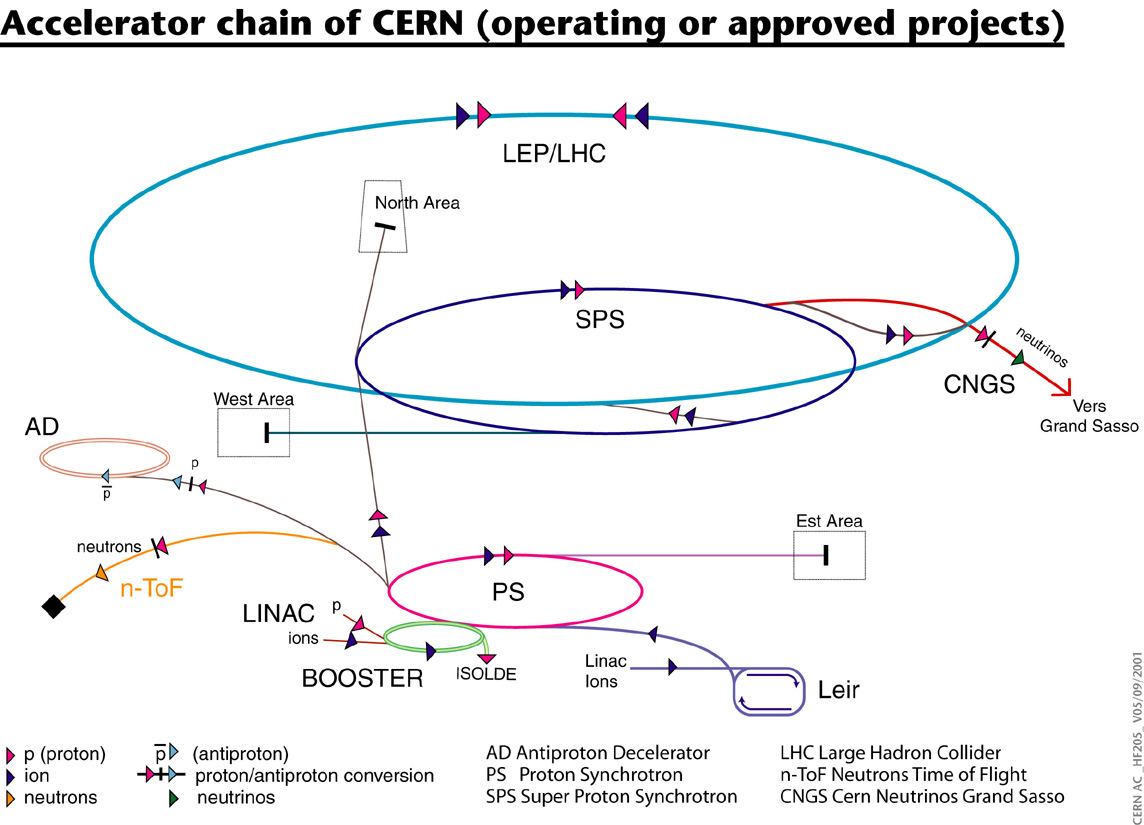
\includegraphics[scale=0.74]{accelerators}
\end{center}
\caption{Diagrama esquemático dos aceleradores do CERN e suas conexões.}
\label{fig:accel}
\end{figure}

\section{O LHC}

No LHC, a energia disponível nas colisões entre os constituintes dos prótons
(\idxeng{quarks} e \idxeng{glúons}) chegará a faixa dos TeV's, o que
representa aproximadamente 10 vezes a potência atingida pelo LEP ou pelo
Tevatron no Fermilab \cite{lhc}. De forma a manter um programa de física
efetivo a uma energia mais alta (digamos, $E$), a luminosidade de um
colisionador, uma quantidade proporcional ao número de colisões por segundo,
deve aumentar proporcionalmente com $E^2$. Isto acontece porque o comprimento
de onda associado à partícula decresce com $1/E$ e, portanto, a seção
transversal da partícula decrescerá com $1/E^2$! Se o tamanho da partícula
decresce, menor a chance de ocorrer uma colisão. Para compensar este efeito,
aumenta-se o número de colisões por base de tempo. Enquanto colisionadores
mais antigos podem atingir uma luminosidade de $L = 10^{32}
\text{cm}^{-2}\text{s}^{-1}$, no LHC este parâmetro será de $L = 10^{34}
\text{cm}^{-2}\text{s}^{-1}$. Este valor será atingido alimentando-se cada um dos
dois anéis com 2835 pacotes de 1011 partículas cada.

Quando dois pacotes cruzam o centro de um detetor, somente uma pequena fração
das partículas colide de forma aproximadamente inelástica, provocando uma
aniquilação bastante eficiente da matéria, para produzir os eventos de
interesse. Todas as outras são defletidas pelo forte campo magnético do outro
pacote. Estas defleções, que são mais intensas para pacotes mais densos,
acumulam-se volta após volta e, com isso, podem eventualmente acarretar em
perda de partículas. Este efeito do feixe foi estudado em colisionadores mais
antigos e a experiência mostrou que não é possível aumentar muito a densidade
do pacote de partículas acima de um limite feixe-feixe para preservar uma vida
útil suficientemente grande para o feixe. Para atingir a luminosidade
desejada, o LHC tem que operar bastante próximo deste limite. Seus injetores,
o antigo PS e o SPS, estão sendo re-equipados para prover exatamente a
densidade de feixe desejada.

Os feixes do LHC são armazenados por aproximadamente 10 horas em altas
energias. Durante este período, as partículas fazem 400 milhões de revoluções
ao redor da máquina, um número verdadeiramente astronômico. Enquanto isso, a
amplitude das oscilações ao redor da órbita central não pode aumentar
significativamente, pois isso dissolveria o feixe e degradaria a luminosidade
do colisionador. Isto é bastante difícil de ser atingido já que, além da
interação feixe-feixe mencionada anteriormente, pequenas não-linearidades nos
componentes geradores dos campos magnéticos para a focalização do feixe podem
fazer o movimento se tornar ligeiramente caótico de forma que, depois de
várias voltas, partículas podem ser perdidas. No LHC, os efeitos mais
desestabilizadores das imperfeições magnéticas são produzidos durante a
injeção das partículas no grande anel. Para controlar os estragos deste tipo
de efeito, se utilizam computadores rápidos para rastrear o traçado de
centenas de partículas passo-a-passo, através dos milhares de imãs
espalhados pelo LHC, até completarem cerca de 1.000.000 de voltas,
compensando-se o efeito dos campos para estabilizar o sistema.

Quatro grandes experimentos se basearão no LHC:

\begin{itemize}

\item \idx{\textbf{ALICE}}: estuda a física de matéria com fortes interações
em energias extremamente densas \cite{alice};

\item \idx{\textbf{LHCb}}: para realizar medidas precisas da violação CP e
decaimentos raros \cite{lhcb};

\item \idx{\textbf{ATLAS}} \cite{atlas-site} e \idx{\textbf{CMS}} \cite{cms}:
que estarão basicamente focados na deteção do \idx{bóson de Higgs}, embora
também incluam programas para estudo de outros tipos de Física, como Física B
ou envolvendo íons pesados. Estes detetores são bastante complexos e podem ser
reconfigurados facilmente para estudo de nova física, na remota possibilidade
de não serem encontradas evidências do bóson de Higgs.

\end{itemize}

Uma vez que o LHC será construído sob a superfície (aproximadamente a 100
metros de profundidade), para evitar distúrbios causados pela radiação solar,
estes experimentos serão montados em poços comunicantes com a estrutura do
acelerador. A Figura~\ref{fig:aerial} mostra uma visão esquemática da
fronteira entre Suíça e a França, indicando a localização dos poços dos
experimentos acima, tal como a localização dos domínios do CERN, em
\fr{Meyrin} na Suíça e em \fr{Prevessin} na França.

\begin{figure}
\begin{center}
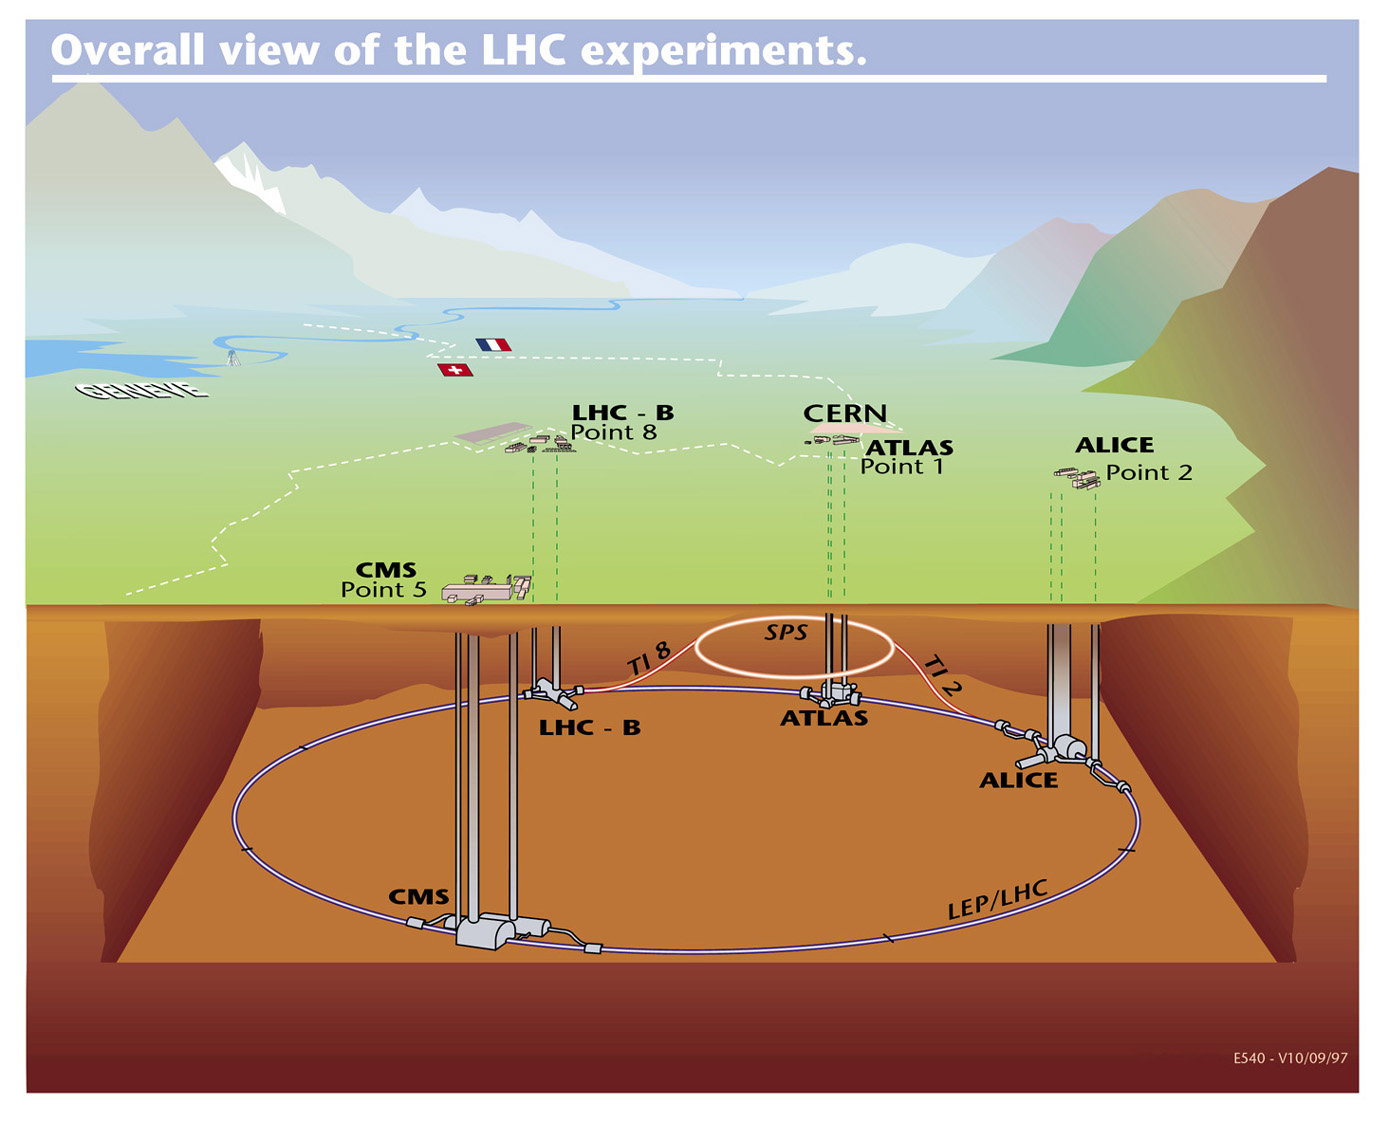
\includegraphics[scale=0.6]{lhc-underground.jpg}
\end{center}
\caption{Visão esquemática da fronteira franco-suíça mostrando o CERN e os
pontos de accesso aos poços dos 4 experimentos do LHC.}
\label{fig:aerial}
\end{figure}

O LHC estará apto a produzir cerca de 40.000.000 milhões de interações por
segundo (ou 40 MHz) e estará dedicado a cada um dos experimentos de forma
alternada com relação a paradas para o enchimento do feixe (do inglês
\idxeng{fill}). Cada período de aquisição programada ou \idxeng{run} durará
cerca de 10 horas. Os experimentos terão este período para adquirir dados e
perseguir o objetivo físico a que se destinam.

\section{O Experimento ATLAS}
\index{ATLAS}

Um dos objetivos principais do experimento ATLAS é descobrir e estudar o
\idx{bóson de Higgs}. Esta partícula tem importância crítica na teoria das
partículas, como destacado no Capítulo~\ref{chap:introducao}, pois está
diretamente ligada ao conceito de ``massa''\index{conceito de massa} e,
portanto, das partículas.

\paragraph{A charada da massa} É interessante notar que um conceito tão
familiar como a massa não era entendido até a proposição do \idx{Modelo
Padrão}. A maioria de nós está familiarizado com campos magnéticos, elétricos
e gravitacionais. Uma pessoa no campo gravitacional da Terra sente a sua
força. Ondas eletromagnéticas viajam pelo espaço da mesma forma que ondas
se propagam sobre água. Se este balanço fosse descrito pela Mecânica Quântica,
a superfície da água que carrega as ondas seria chamada de ``campo''.

O Modelo Padrão propõe que exista um outro campo ainda não observado, um campo
que é praticamente indistingüível do espaço vazio. Este campo é normalmente
chamado de \idx{campo de Higgs}. Acredita-se que todo o espaço seja preenchido
com este campo e, interagindo com ele, partículas adquirem suas
massas. Partículas que interajam fortemente com o campo são pesadas, enquanto
que aquelas que interajam fracamente tornam-se mais leves.

O campo de Higgs tem ao menos uma nova partícula associada a ele - o bóson de
Higgs. O detetor ATLAS será capaz de detetar esta partícula, se existir,
tornando-se uma das maiores descobertas físicas de todos os tempos.

\section{O Detetor ATLAS}

O detetor ATLAS é um aparato em formato cilíndrico, capaz de registrar os
subprodutos de colisões próton-antipróton a 40 MHz. A
Figura~\ref{fig:atlas-scheme} mostra um esquema do detetor. Repare na parte
inferior à direita, em escala, o tamanho proporcional das pessoas.

\begin{figure}
\begin{center}
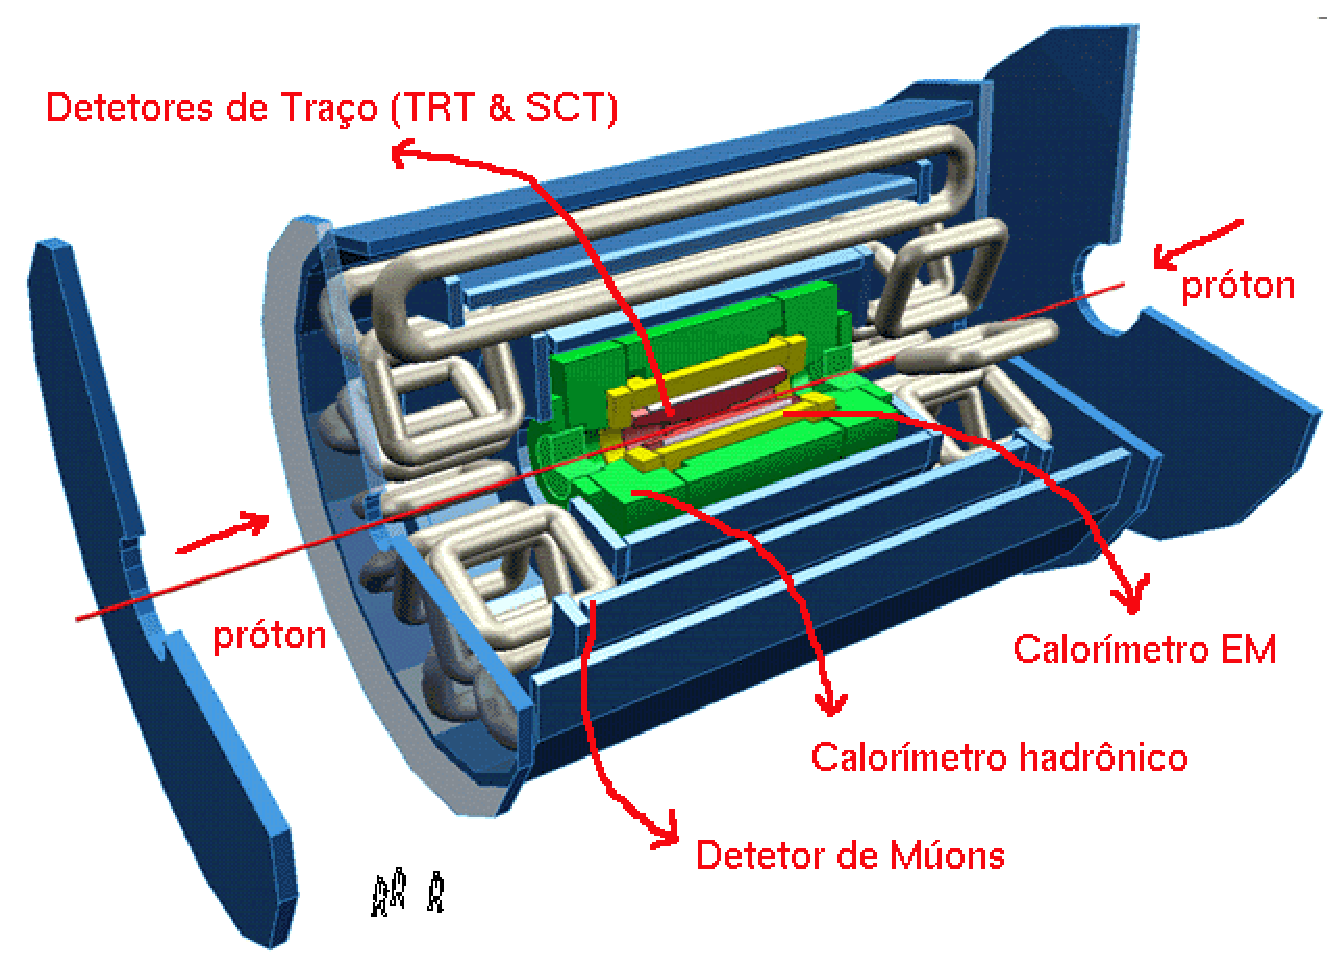
\includegraphics[scale=0.65]{atlas-andre}
\end{center}
\caption{O detetor ATLAS.}
\label{fig:atlas-scheme}
\end{figure}

O detetor \idx{ATLAS} é composto, como mostra a figura, de 4 sistemas de
deteção independentes. Na parte mais interna, encontram-se detetores de traço
altamente segmentados, que podem medir a trajetória de partículas
carregadas. Ao redor deste sistema, ficará instalado a seção eletromagnética
do calorímetro. Em seguida, vemos a seção hadrônica dos calorímetros do ATLAS
e, finalmente, englobando toda a estrutura, detetores de múons. A posição do
feixe com relação ao detetor também é destacada na figura.

\subsection{Os Detetores de Traços}
\index{detetores de traços}
\label{sec:atlas-id}

O papel do \idx{Detetor Interno} (do inglês \idxeng{Inner Detector}, ID) é
reconstruir traços e vértices de um evento com alta eficiência conjuntamente
ao calorímetro (veja a Seção~\ref{sec:atlas-calo}) e aos detetores de múons
(veja a Seção~\ref{sec:atlas-muon}), para o reconhecimento de elétrons, fótons
e múons e suprindo assinaturas extras para vértices provenientes de partículas
que decaem rapidamente \cite{atlas-id-tdr}. Sua aceitação cobre a região de
\idx{pseudo-rapidez} (veja o Apêndice~\ref{ap:coord}) de $\pm2,5$, igualando,
em alcance, o restante dos sistemas do detetor ATLAS.

A Figura~\ref{fig:atlas-id-3d} mostra um corte tridimensional do ID. Este
sistema combina detetores de alta resolução na parte interna com elementos
para a deteção de traços em modo contínuo, na parte externa, todos envolvidos
por um \idx{solenóide} com campo central de 2 Tesla.

\begin{figure}
\begin{center}
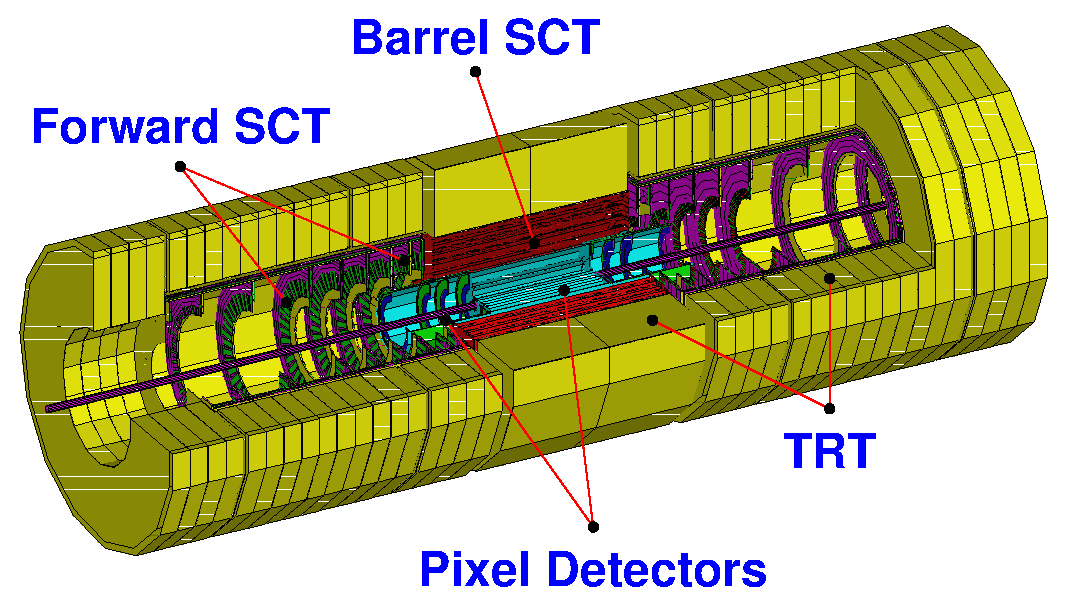
\includegraphics[scale=0.8]{inner_3D}
\end{center}
\caption{Corte tridimensional do Detetor Interno do ATLAS.}
\label{fig:atlas-id-3d}
\end{figure}

Os alvos de momento e resolução de vértices requerem que medições de alta
precisão sejam feitas com detetores de alta segmentação, dada a grande
densidade de traços esperada em experimentos ao redor do LHC. \idx{Detetores
de traços baseados em semi-condutores} (do inglês, \idxeng{Semi-Conductor
Tracker}, \idx{SCT}), usando pastilhas\index{SCT!pastilhas} e
pontos\index{SCT!pontos} (ou \idxeng{pixels}) microscópicos de silício
oferecem estas características e, portanto, esta tecnologia é utilizada na
parte mais interior do ID. Entretanto, o número total de camadas de precisão
deve ser limitado por causa do excesso de matéria que estes detetores
introduzem e do seu alto custo. Segundo o projeto do ID, a trajetória das
partículas cruzará, na pior das hipóteses, 4 camadas com sensores em formato
de pastilhas e 3 camadas com sensores em pontos de silício.

Um grande número de pontos da trajetória (tipicamente 36 por traço) será
detetado por um \idx{Detetor de traços em microtubos} (do inglês,
\idxeng{Straw Tube Tracker}, \idx{TRT}) que provê a possibilidade do
acompanhamento das trajetórias em modo contínuo com uma quantidade muito menor
de material por ponto e baixo custo. A combinação destas duas técnicas
propicia um reconhecimento de trajetórias bastante robusto e com alta
precisão, tanto em $\phi$ como em $z$ (veja a definição completa no
Apêndice~\ref{ap:coord}. A sensibilização dos microtubos na parte
exterior do detetor contribuirá para a deteção do momento da partícula, onde a
baixa precisão do sistema, se comparado com o SCT, é compensada pelo grande
número de pontos medidos numa maior seção do espaço.

\subsection{Os Calorímetros}
\index{calorímetros}
\label{sec:atlas-calo}

Os calorímetros desempenham um papel central na arquitetura do experimento
ATLAS \cite{atlas-calo-tpr}. Estes detetores foram projetados para contribuir
ativamente na filtragem de física interessante e na medição precisa de
elétrons, fótons, jatos e \idx{energia transversa perdida} (do inglês
\idxeng{missing $E_{T}$}) no difícil ambiente do LHC, trabalhando na sua
máxima luminosidade.

O sistema pode ser caracterizado funcionalmente ou
arquiteturalmente. Funcionalmente é possível classificar os calorímetros do
ATLAS em:

\begin{itemize}
\item \textbf{Eletromagnético ou e.m.}: Para a deteção de partículas que
desenvolvem cascatas e.m. como elétrons ou fótons, situando-se na parte mais
interior da estrutura;

\item \textbf{Hadrônico}: Para a deteção de partículas ou jatos que
desenvolvam cascatas baseadas em hádrons, como nêutrons, prótons e píons.

\item \textbf{\idx{Avançado} ou \idxeng{Forward}}: Para a deteção de partículas
próximas ao eixo do feixe de colisão. Estes dispositivos tendem a ser menos
precisos uma vez que a física envolvida nestes ângulos de pseudo-rapidez
normalmente não representam processos de interesse. Este calorímetro não será
abordado neste trabalho, em nenhum de seus níveis, uma vez que é comumente
utilizado somente para efeitos de análise \eng{off-line}.
\end{itemize}

Com relação à arquitetura dos calorímetros, é possível classificar os
detetores da seguinte forma:

\begin{itemize}
\item \textbf{\idx{Argônio Líquido} com \idx{eletrodos de chumbo}}: É um
calorímetro que utiliza o Argônio Líquido como material absorvedor e eletrodos
de chumbo para captar os íons formados durante a interação da partícula com
seu volume. Os eletrodos são dispostos em forma de "acordeão", o que confere a
esta estrutura um formato peculiar. Esta tecnologia foi escolhida para a maior
parte do sistema, cobrindo toda a seção e.m., as tampas hadrônicas e para o
calorímetro avançado \cite{lar-tdr}.

\item \textbf{\idx{Telhas Cintilantes} ou \idxeng{Tiles}}: É um
calorímetro de amostragem que utiliza uma liga de aço como material absorvedor
e telhas cintilantes\footnote{Diz-se cintilante o material que emite luz
quando uma partícula cruza seu volume. A luz emitida é proporcional à energia
da partícula que passa.} como elemento amostrador. Esta técnica foi escolhida
somente para a seção hadrônica do barril \cite{tilecal}.
\end{itemize}

A Figura~\ref{fig:calo-general} mostra uma esquematização dos calorímetros do
ATLAS, indicando as partes mencionadas.

\begin{figure}
\begin{center}
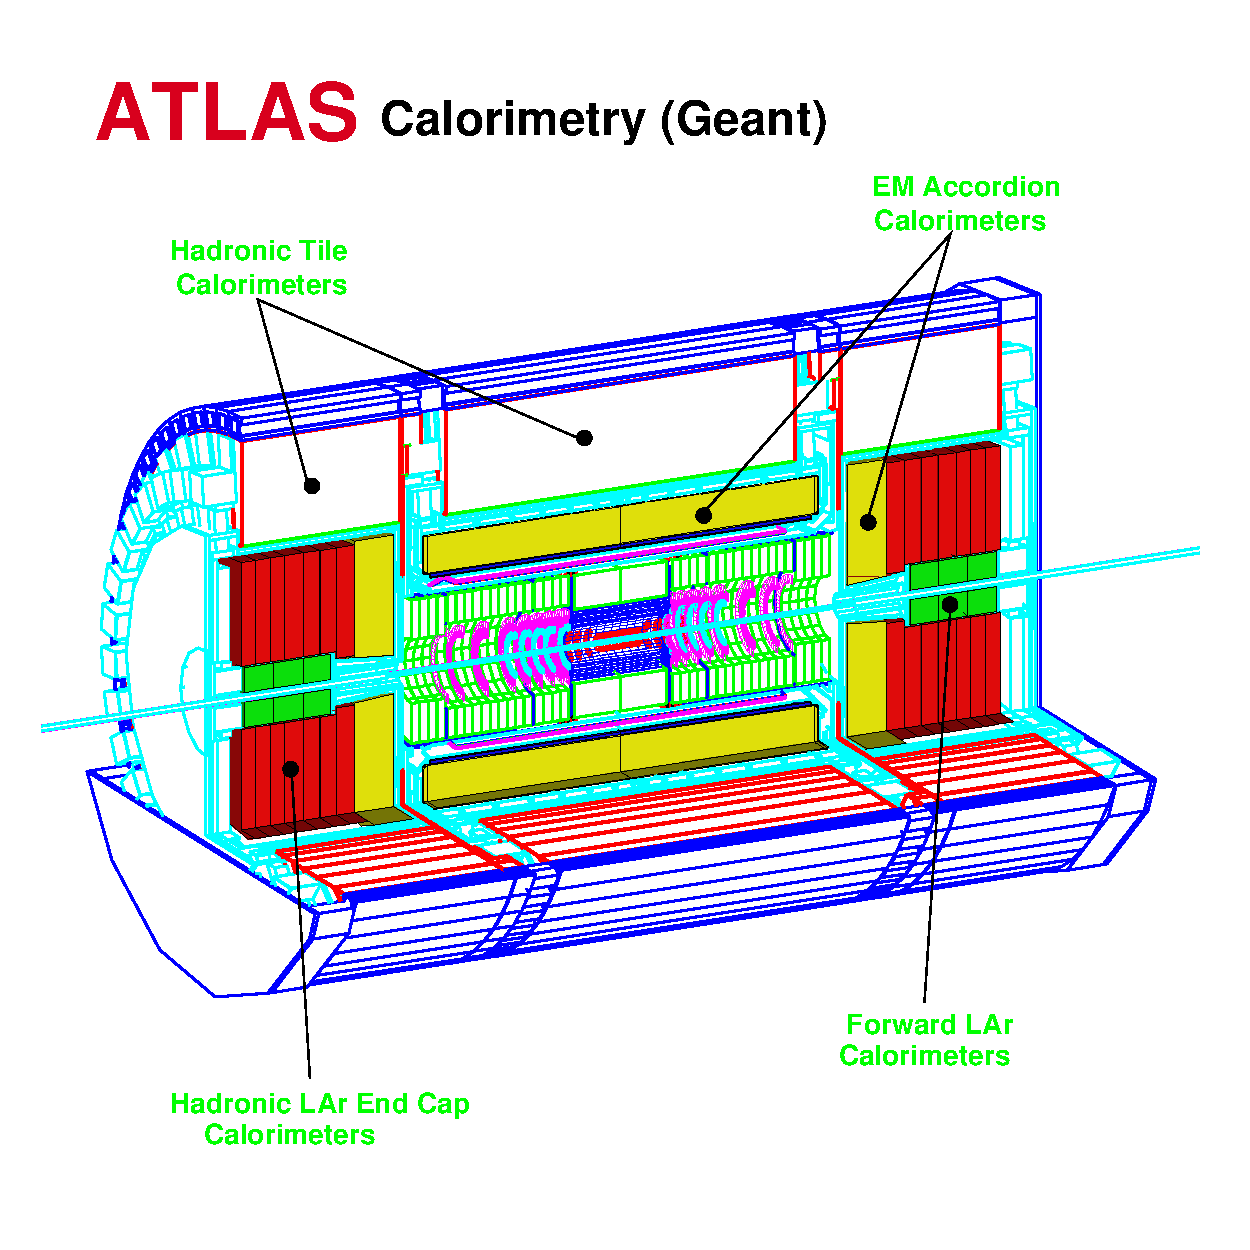
\includegraphics[scale=0.7]{atlas-calorimetry}
\end{center}
\caption{Diagrama esquemático dos calorímetros no detetor ATLAS.}
\label{fig:calo-general}
\end{figure}

\subsubsection{A Seção E.M.}

A seção e.m. do ATLAS é divida em 3 camadas, das quais a segunda é a mais
profunda. Cada camada possui uma segmentação\footnote{A ``segmentação"\ de um
detetor é a resolução deste no plano $\eta\times\phi$.} específica que otimiza
a relação custo-benefício do detetor. As camadas mais internas são mais
segmentadas, permitindo a localização precisa das partículas no plano
$\eta\times\phi$, enquanto as mais externas são concebidas de forma menos
segmentada e mais profunda, com o objetivo de absorver toda a energia da
partícula incidente, limitando os custos de produção. 

A seção e.m. é divida em três partes: o barril (do inglês
\eng{barrel}) e duas tampas (\eng{endcap}). Estas partes fecham quase que
hermeticamente o espaço ao redor da colisão até um valor de $|\eta|=3,2$ (para
maiores referências sobre o sistema de coordenadas do ATLAS, leia o
Apêndice~\ref{ap:coord}). A Figura~\ref{fig:lar-pos} mostra o posicionamento
do calorímetro eletromagnético no detetor ATLAS. Sua segmentação não é
mostrada nesta figura. Ao invés, mostram-se os valores de $\eta$ que definem
os limites geométricos da seção e.m.. Pode-se perceber que a porção do barril
de tal calorímetro estende-se de $\eta=0$ até $|\eta|=1,475$. Em
$|\eta|=1,375$, o barril começa a sobrepor a tampa, que é dividida entre tampa
exterior (até $|\eta|=2,5$) e interior (de $|\eta|=2,5$ até $|\eta|=3,2$).

\begin{figure}
\begin{center}
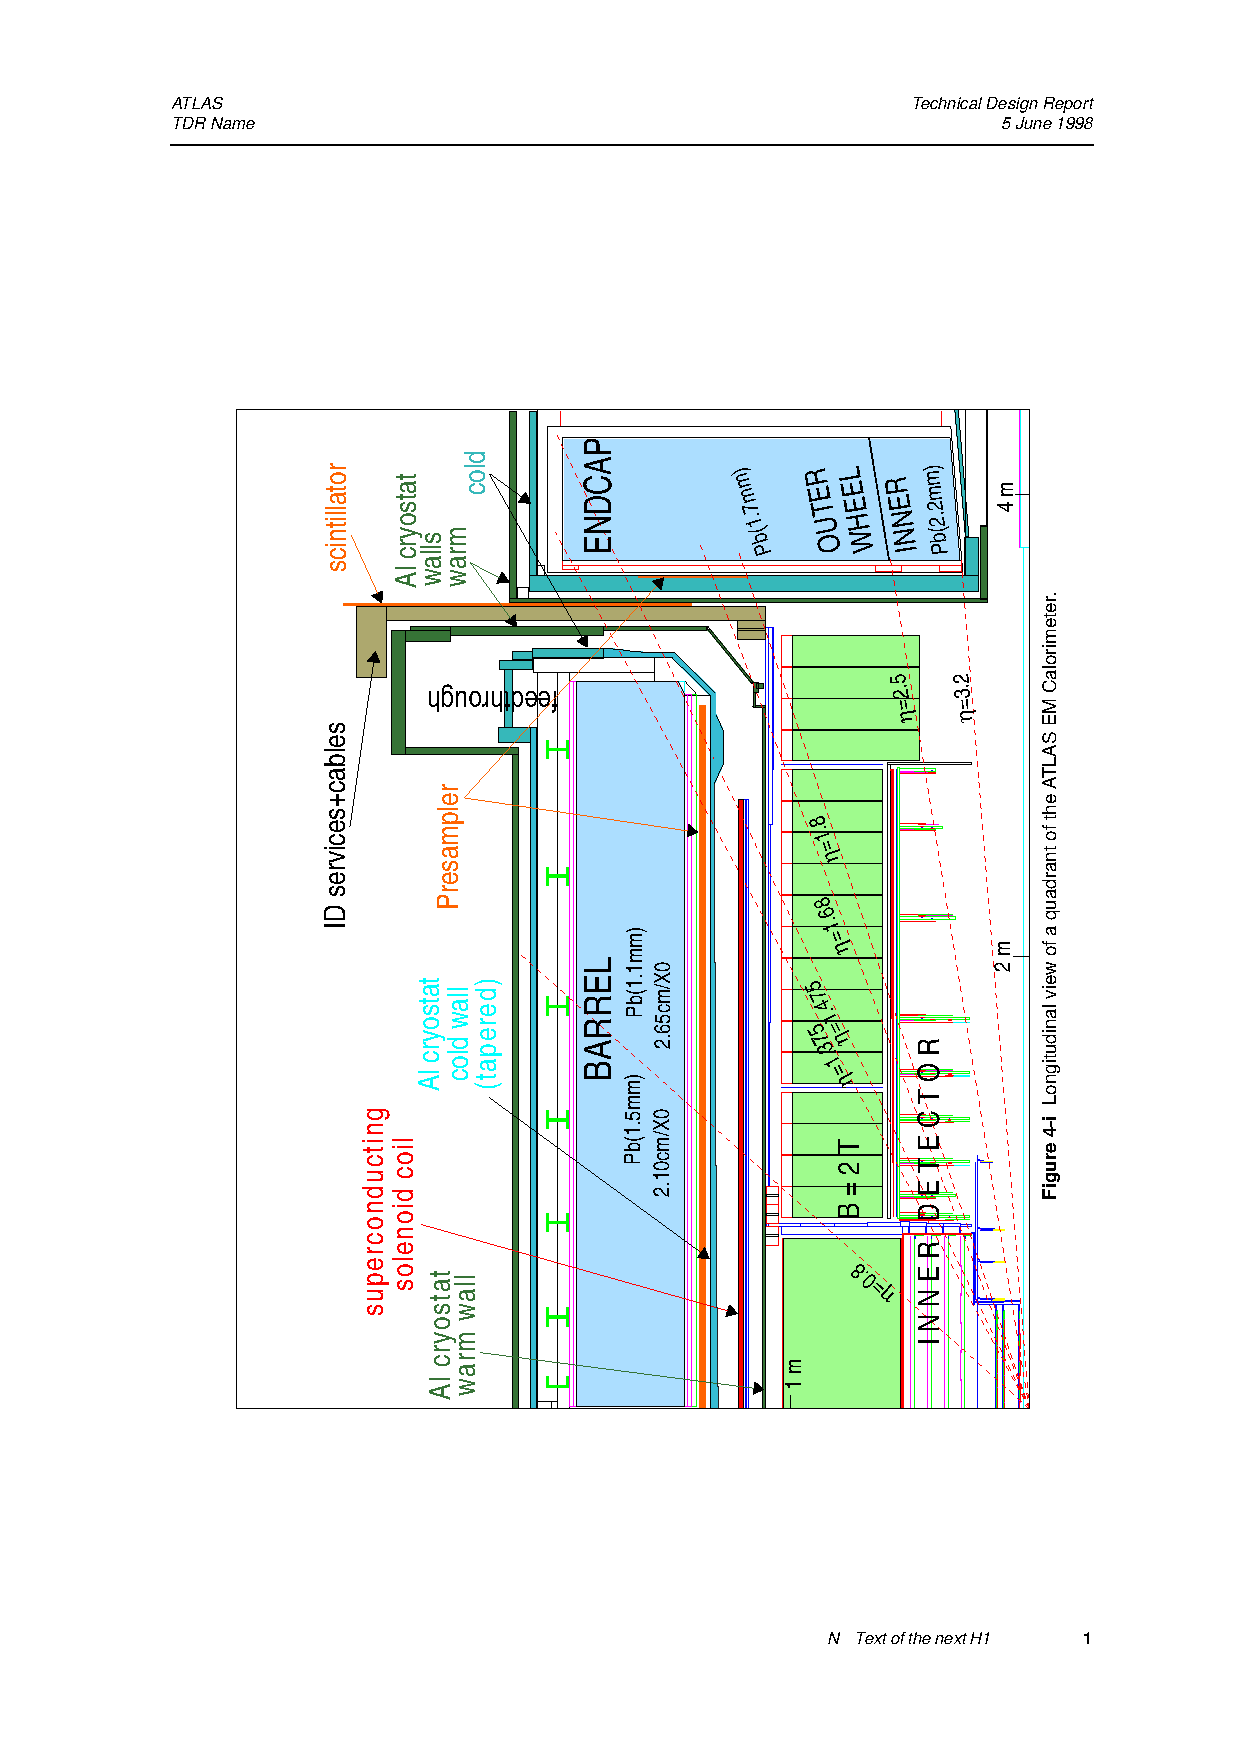
\includegraphics[scale=0.6]{lar-detail}
\end{center}
\caption{O Calorímetro e.m. do ATLAS em um corte transversal.}
\label{fig:lar-pos}
\end{figure}

O calo\-rí\-metro e.m. do ATLAS tam\-bém inclui um pré-irradiador (do inglês,
\eng{pre-sampler}), que funciona praticamente como um calo\-rí\-metro muito
fino, posicionado antes dos calo\-rí\-metros de ar\-gô\-nio lí\-quido, com a
função de recuperar a informação perdida no material \textit{morto} da seção
e.m. (ou seja, fios, encapamentos, etc.). O pré-irradiador pode ser observado,
na figura, de $\eta=0$ até $|\eta|=1,5$ no barril, e depois, de $|\eta|=1,5$
até $|\eta|=1,8$ nas tampas.

Uma observação mais apurada da Figura~\ref{fig:lar-pos} revela um
\textit{buraco} entre o barril e a tampa da seção e.m.. Esta falha existe para
que seja possível passarem-se os cabos acoplados aos sensores do ID. Para que
a perda nessa região seja minimizada, decidiu-se por colocar um cintilador
(indicado na figura). Cintiladores são detetores que se excitam pela passagem
das partículas energéticas e produzem luz. Cintiladores são normalmente
bastante compactos e finos.

\paragraph{Segmentação da seção e.m.} O calorímetro e.m. do ATLAS possui
uma segmentação constante com relação à rotação (eixo $\phi$), mas variável
com relação ao eixo $\eta$. Este calorímetro é dividido em 3 camadas, com
segmentações independentes. Isto quer dizer que ao longo do eixo z, a
segmentação pode variar. A Figura~\ref{fig:lar-detail} exemplifica a
diversificação da segmentaçao ao longo do eixo $\phi$. Cada camada é formada
por células de diferentes tamanhos. Nesta figura, também se verifica que a
segunda camada é a que possui células mais profundas. É plausível esperar que
mais energia seja amostrada nesta camada.

\begin{figure}
\begin{center}
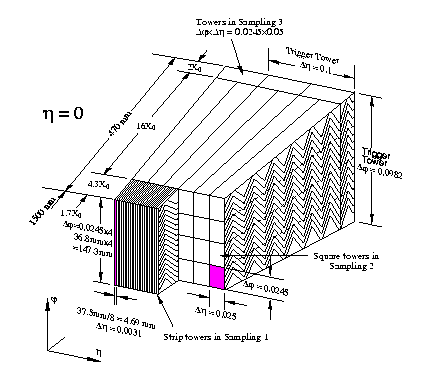
\includegraphics[scale=0.95]{lar-square}
\end{center}
\caption{Diagrama de um dos gomos do barril da seção e.m. do ATLAS.}
\label{fig:lar-detail}
\end{figure}

A Tabela~\ref{tab:lar} resume as informações de segmentação para a seção e.m.,
incluindo informações sobre o \eng{pre-sampler} e as tampas. Nota-se, a partir
da tabela, que a segmentação de algumas camadas varia bastante com $\eta$. A
coluna da extrema direita indica o número de células numa área de
$0,1\times0,1$ no plano $\eta\times\phi$. Esta área é uma referência para os
níveis de filtragem, como será visto mais adiante.

\begin{table}
\caption{A segmentação, camada a camada, dos calo\-rí\-metros e.m. do ATLAS.}
\label{tab:lar}
\index{calorímetro!e.m.!segmentação}
\begin{center}
%% Hello emacs, this is -*- latex -*-
\typeout{ ====================================================================}
\typeout{ This is file em-grains.tex, created at 25-Feb-2004 }
\typeout{ Maintained by Andre DOS ANJOS <Andre.dos.Anjos@cern.ch> }
\typeout{ ====================================================================}

\begin{tabular}{||l||l||c||c||c||c||} 
\hhline{|t:=:t:=:t:=:t:=:t:=:t:=:t|}
Camada & Peça & $\eta_{\text{início}}$ & $\eta_{\text{fim}}$& 
$\Delta\eta \times \Delta\phi$& $ N_{\eta} \times N_{\phi} $ \\ 
\hhline{|:=::=::=::=::=::=:|}
\multirow{2}{70pt}{\eng{Pre-sampler}} & Barril & 0 & 1,5 &
	$0,025\times0,1$ & $4 \times 1$\\ 
\hhline{||~||-||-||-||-||-||}
& Tampa & 1,5 & 1,8 & 
	$0,025\times0,1$ & $4 \times 1$ \\ \hhline{|:=::=::=::=::=::=:|}

\multirow{8}{70pt}{Camada 1} & \multirow{2}{40pt}{Barril} & 0& 1,4&
	$0,003125\times1$& $32 \times 1$\\
                  	    & & 1,4 & 1,475 & 
	$0,025\times0,025$& $4 \times 4$ \\
\hhline{||~||-||-||-||-||-||}
& \multirow{6}{70pt}{Tampa} & 1,375& 1,5& $0,025\times0,1$& $1 \times 4$\\
& & 1,5& 1,8& $0,003125\times0,1$& $32 \times 1$\\
& & 1,8& 2,0& $0,004167\times0,1$& $24 \times 1$\\
& & 2,0& 2,4& $0,00625\times0,1$& $16 \times 1$\\
& & 2,4& 2,5& $0,025\times0,1$& $4 \times 1$\\
& & 2,5& 3,2& $0,1\times0,1$& $1 \times 1$\\ \hhline{|:=::=::=::=::=::=:|}

\multirow{4}{70pt}{Camada 2} & \multirow{2}{40pt}{Barril} & 0& 1,4& 
	$0,025\times0,025$& $4 \times 4$\\
		             & & 1,4 & 1,475 & $0,075\times0,025$& $1\times4$\\
\hhline{||~||-||-||-||-||-||}
                             & \multirow{2}{40pt}{Tampa} & 1,375& 2,5& 
	$0,025\times0,025$ & $4 \times 4$\\
			     & & 2,5& 3,2& $0,1\times0,1$ & $1 \times 1$\\
\hhline{|:=::=::=::=::=::=:|}

\multirow{2}{70pt}{Camada 3} & Barril & 0& 1,35& 
$0,05\times0,025$ & $2 \times 4$\\ \hhline{||~||-||-||-||-||-||} 
& Tampa & 1,5 & 2,5& $0,05\times0,025$ & $2 \times 4$\\
\hhline{|b:=:b:=:b:=:b:=:b:=:b:=:b|}

\end{tabular}

\typeout{ *************** End of file em-grains.tex *************** }

\end{center}
\end{table}

\subsubsection{A Seção Hadrônica}

Os calorímetros hadrônicos do ATLAS são formados pelo \idx{Calorímetro de
Telhas} ou \idxeng{TileCal} e pela Tampa Hadrônica baseada em Argônio Líquido
- a mesma técnica usada para a seção e.m.. O TileCal é um calorímetro de
amostragem cujo material absorvedor é uma liga com aço e os elementos
amostradores são telhas cintilantes \cite{tilecal}. As telhas são posicionadas
em planos perpendiculares aos feixes de partículas colididas e conectadas a
fibras ópticas em duas de suas extremidades. Estas fibras coletam o sinal
luminoso, gerado pela telha ao interagir com a partícula, e transportam-no até
tubos fotomultiplicadores (PM)\index{tubos fotomultiplicadores}, onde o sinal
é convertido em sinal elétrico. Somadores rápidos \cite{seixas:adder} se
encarregam de adicionar os sinais das telhas entre si formando células de
deteção, de forma equivalente à seção e.m.. O TileCal é posicionado após a
seção e.m., como é possível verificar na Figura~\ref{fig:tile-pos}.

\begin{figure}
\begin{center}
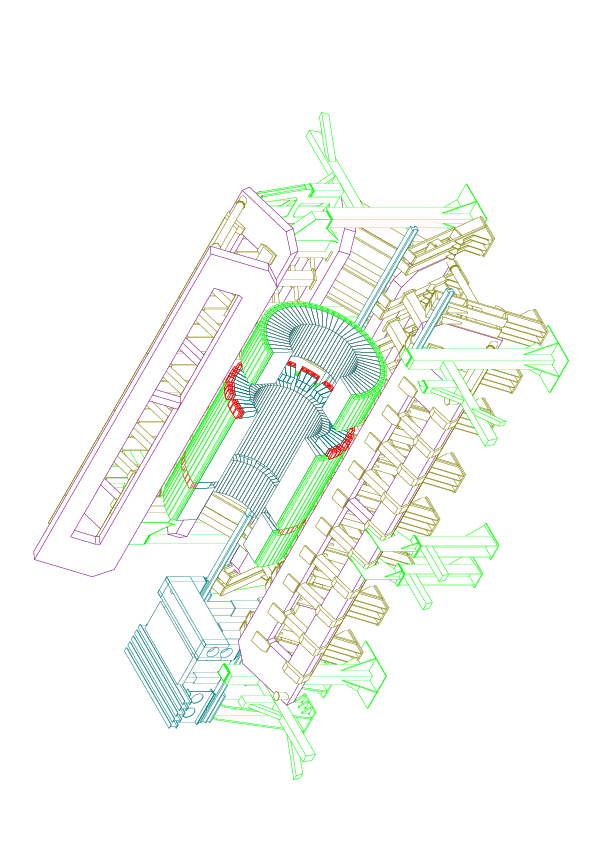
\includegraphics[scale=0.5,angle=-90]{tilecal-3d}
\end{center}
\caption{O calorímetro de telhas do ATLAS (em verde ao centro), em sua posição
final, envolvido pelo detetor de múons (em roxo e marrom).}
\label{fig:tile-pos}
\end{figure}

Uma peculiaridade dos calorímetros hadrônicos do ATLAS é que o barril e a
tampa são feitos de formas diferentes, ao contrário da seção e.m.. O
calorímetro de telhas (TileCal) abrange as porções do barril ($0<|\eta|<1,0$)
e sua extensão ($0,8<|\eta|<1,7$). A tampa desta seção é feita como os
calorímetros e.m., no formato de acordeões, usando Argônio líquido.

A Tabela~\ref{tab:had} resume a informação de segmentação da seção hadrônica
dos calorímetros do ATLAS, de forma equivalente a da Tabela~\ref{tab:lar}.
Nessa tabela é possível perceber que o tamanho das células, em média, é bem
maior que o valor equivalente no calorímetro eletromagnético. A segmentação
é também mais uniforme que na seção e.m. dos calorímetros do ATLAS. Isto se
deve ao fato dos chuveiros hadrônicos serem mais largos e profundos,
provocando maiores flutuações nas medidas de energia e, portanto, não
necessitando de uma segmentação tão fina.

Outra diferença é na área de referência. Na seção e.m., considera-se
$0,1\times0,1$ - aqui a área de referência é de $0,2\times0,2$, já que se
encontram células maiores que a área de referência no calorímetro e.m..

\begin{table}
\caption{A segmentação, camada a camada, dos calo\-rí\-metros ha\-drô\-nicos
do ATLAS.}
\label{tab:had}
\index{calorímetro!hadrônico!segmentação}
\begin{center}
%% Hello emacs, this is -*- latex -*-
\typeout{ ====================================================================}
\typeout{ This is file had-grains.tex, created at 25-Feb-2004 }
\typeout{ Maintained by Andre DOS ANJOS <Andre.dos.Anjos@cern.ch> }
\typeout{ ====================================================================}

\begin{tabular}{||l||l||c||c||c||c||} 
\hhline{|t:=:t:=:t:=:t:=:t:=:t:=:t|}
Camada& Pe�a & $\eta_{\text{in�cio}}$ & $\eta_{\text{fim}}$& 
$\Delta\eta \times \Delta\phi$& $ N_{\eta} \times N_{\phi} $ \\ 
\hhline{|:=::=::=::=::=::=:|}
\multirow{4}{50pt}{Camadas 1 e 2} & Barril (TileCal)& 0 & 1,0 & 
	$0,1\times0,1$ & $2\times2$ \\
\hhline{||~||-||-||-||-||-||}
				  & Barril Ext. (TileCal)& 0,8 & 1,7 & 
	$0,1\times0,1$ & $2\times2$ \\
\hhline{||~||-||-||-||-||-||}
	& \multirow{2}{60pt}{Tampa (LAr)} & 1,5 & 2,5 &
	$0,1\times0,1$ & $2\times2$ \\
	&                           & 2,5 & 3,2 & 
	$0,2\times0,2$ & $1\times1$ \\

\hhline{|:=::=::=::=::=::=:|}

\multirow{4}{50pt}{Camada 3} & Barril (TileCal)& 0 & 1,0 & 
	$0,2\times0,1$ & $1\times2$ \\
\hhline{||~||-||-||-||-||-||}
				  & Barril Ext. (TileCal)& 0,8 & 1,7 & 
	$0,2\times0,1$ & $1\times2$ \\
\hhline{||~||-||-||-||-||-||}
	& \multirow{2}{60pt}{Tampa (LAr)} & 1,5 & 2,5 & 
	$0,1\times0,1$ & $2\times2$ \\
	&                           & 2,5 & 3,2 & 
	$0,2\times0,2$ & $1\times1$ \\

\hhline{|b:=:b:=:b:=:b:=:b:=:b:=:b|}

\end{tabular}

\typeout{ *************** End of file had-grains.tex *************** }

\end{center}
\end{table}

A Figura~\ref{fig:tilecell} mostra uma seção transversal da parte do Barril do
Calorímetro de Telhas. Nesta figura, verifica-se que o sistema de leitura
agrupa as células deste detetor em 3 camadas. A segmentação no sentido de
$\eta$ é mantida constante ainda assim.

\begin{figure}
\begin{center}
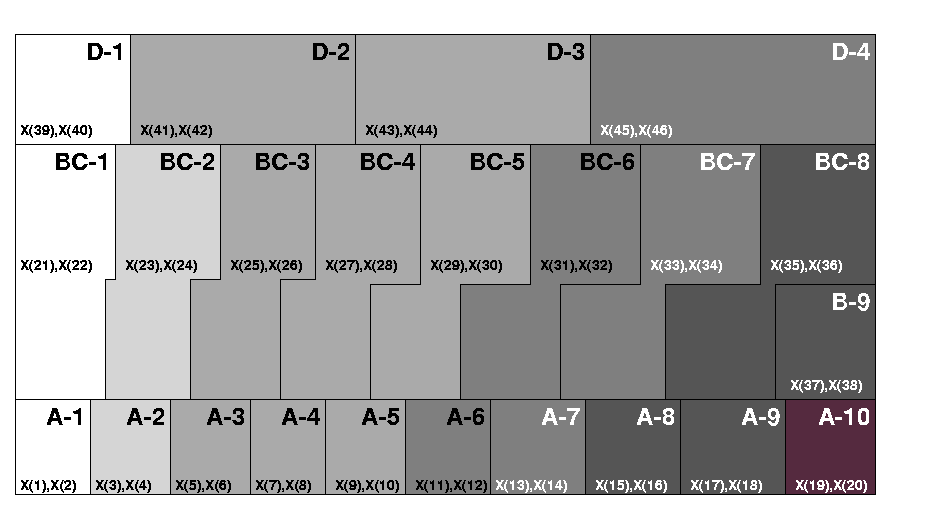
\includegraphics[scale=0.5]{tilecell}
\end{center}
\caption{Configuração de leitura das células da seção do barril do Calorímetro
de Telhas.}
\label{fig:tilecell}
\end{figure}

\subsection{O Detetor de Múons}
\index{detetor de múons}
\label{sec:atlas-muon}

\idx{Múons} com grande momento são \idx{assinaturas} bastante
promissoras e robustas da física de interesse no LHC. Para explorar este
potencial, foi projetado um spectrômetro de múons (veja a
Figura~\ref{fig:atlas-muon-3d}) com sistemas de filtragem e medição de momento
com alta resolução independentes do restante do sistema, sensível a este tipo
de partículas \cite{atlas-mu-tdr}. A deteção é baseada na deflexão (magnética)
de múons provida por um grande toróide com núcleo a ar e detetores de traço
bastante precisos. Para $|\eta| \leq 1,0$, um grande magneto em formato de
barril será construído com oito molas circundando a seção hadrônica dos
calorímetros. Para $1,4 \leq |\eta| \leq 2,7$, a deflexão será garantida por
magnetos na forma de tampas ao redor do barril. Esta configuração provê um
campo magnético praticamente transversal à trajetória de eventuais múons.

\begin{figure}
\begin{center}
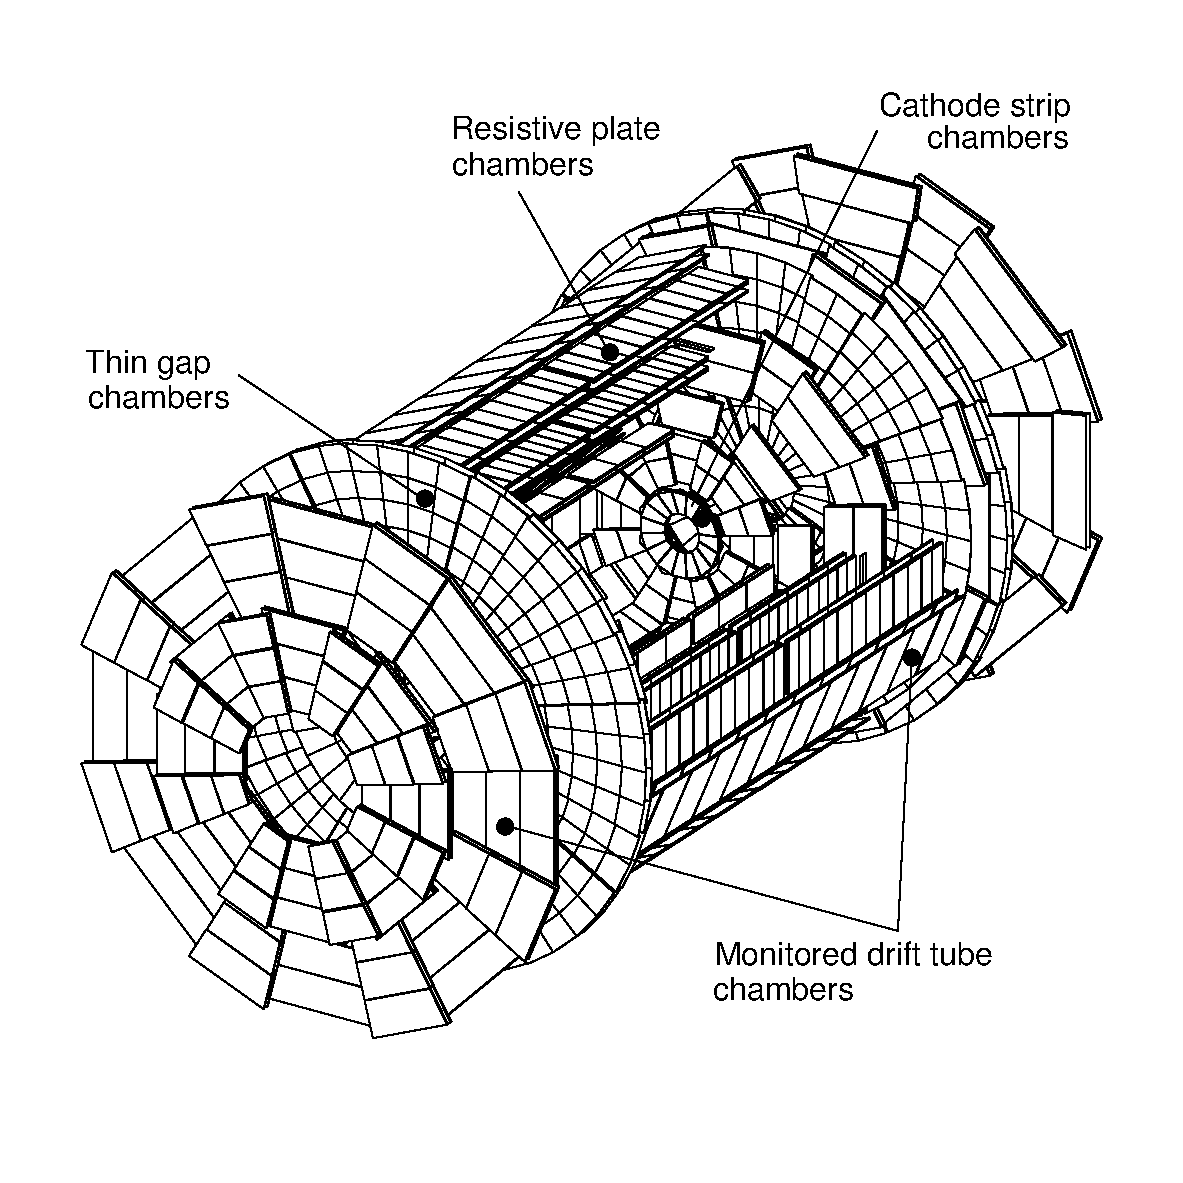
\includegraphics[scale=0.7]{muon-detector}
\end{center}
\caption{Visão tridimensional dos detetores de múons do ATLAS.}
\label{fig:atlas-muon-3d}
\end{figure}

Na região do barril, as trajetórias serão detetadas por câmeras organizadas em
três camadas cilíndricas (estações) ao redor do eixo de colisão. Na região da
tampa, as câmaras serão montadas verticalmente, também em número de três. As
coordenadas dos traços é medida precisamente por \idx{Câmaras de Traços
Monitoradas} (do inglês, \idxeng{Monitored Drift Chambers}, MDT) na direção
principal de deflexão do campo magnético, na maior parte do campo da
pseudo-rapidez. Para grandes valores de pseudo-rapidez, \idx{Câmaras de
Pastilhas Catódicas} (do inglês, \idxeng{Cathode Strip Chambers}, CSC) com
alta segmentação serão construídas para garantir a precisão da deteção nesta
área bastante ruidosa. Tal como os calorímetros, o Spectrômetro de Múons está
diretamente acoplado ao primeiro nível do sistema de filtragem de eventos do
ATLAS (Veja o Capítulo~\ref{chap:trigger}).

\typeout{ *************** End of file atlas.tex *************** }
